\documentclass{standalone}
\usepackage{tikz}

\begin{document}

% description: draw a star with relative coordinates
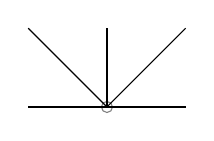
\begin{tikzpicture}
\draw[gray] (0,0) circle [radius=2pt];
\draw (0,0) 

% start
% relative coordinate, 
% without changing current position
edge +(0,1) 
edge +(1,0)
edge +(1,1)
edge +(-1,1)
edge +(-1,0)
%...
;
% end

\end{tikzpicture}

\end{document}
